\section{Diferenciales Exactas}

\begin{ejercicio} \label{ej:3.1}
    Calcula, si es posible, una función potencial para las siguientes parejas de funciones. Especifica en cada caso el
    dominio en el que se trabaja.
    \begin{enumerate}
        \item $P(x, y) = x + y^3$, $Q(x, y) = \nicefrac{x^2}{2} + y^2$.
        
        En este caso, $\Omega=\bb{R}^2$, que trivialmente es convexo y por tanto estrellado. Además, $P,Q\in C^1(\Omega)$ al ser polinomios. Veamos ahora si se cumple la condición de exactitud:
        \begin{equation*}
            \frac{\partial P}{\partial y}(x,y) = 3y^2 \qquad
            \frac{\partial Q}{\partial x}(x,y)= x
        \end{equation*}

        Por tanto, como no se tiene que $\frac{\partial P}{\partial y}(x,y)=\frac{\partial Q}{\partial x}(x,y)$ para todo $(x,y)\in\Omega$, no se da la condición de exactitud y no existe por tanto una función potencial para el campo vectorial $(P,Q)$.
        \item $P(x, y) = \nicefrac{1}{2} \sen 2x - xy^2$, $Q(x, y) = y(1 - x^2)$
        
        En este caso, $\Omega=\bb{R}^2$, que trivialmente es convexo y por tanto estrellado. Además, $P,Q\in C^1(\Omega)$ al ser composición, suma y producto de funciones de clase $1$. Veamos ahora si se cumple la condición de exactitud:
        \begin{equation*}
            \frac{\partial P}{\partial y}(x,y) = -2xy = \frac{\partial Q}{\partial x}(x,y)
        \end{equation*}

        Por tanto, existe una función potencial para este campo vectorial. Para encontrarla, como se busca que $\dfrac{\partial U}{\partial y}=Q$, tenemos que:
        \begin{equation*}
            U(x,y)=\int Q(x,y)dy =
            \int y(1-x^2)dy = \frac{y^2}{2}(1-x^2)+\varphi(x)
        \end{equation*}
        donde $\varphi:\bb{R}\to\bb{R}$ es una función que depende solo de $x$ y representa la constante de integración. Derivando $U$ respecto de $x$ obtenemos:
        \begin{align*}
            \frac{\partial U}{\partial x}(x,y)&=\frac{-2xy^2}{2}+\varphi'(x)\\
            \frac{\partial U}{\partial x}(x,y)&=P(x,y)=-xy^2+\nicefrac{1}{2}\sen 2x
        \end{align*}

        Por tanto, $\varphi'(x)=\nicefrac{1}{2}\sen 2x$. Entonces (y eligiendo como constante de integración $0$ por ser el potencial único salvo una constante aditiva):
        \begin{equation*}
            \varphi(x)=\int \frac{1}{2}\sen 2xdx=-\frac{1}{4}\cos 2x
        \end{equation*}

        Por tanto, la función potencial es (salvo una constante aditiva):
        \begin{equation*}
            U(x,y)=\frac{y^2}{2}(1-x^2)-\frac{1}{4}\cos 2x
        \end{equation*}

        \item \label{ej:3.1c} $P(x, y) = \sqrt{x+y}+\sqrt{x-y}$, $Q(x, y) = \sqrt{x+y}-\sqrt{x-y}$.
        
        Estudiemos en este caso el dominio $\Omega$, que no es trivial. Para que $P,Q\in C^1(\Omega)$, necesitamos que:
        \begin{equation*}
            \Omega=\{(x,y)\in\bb{R}^2 \mid x> y\}\cap\{(x,y)\in\bb{R}^2 \mid x> -y\}
            = \{(x,y)\in\bb{R}^2 \mid x>0, -x< y< x\}
        \end{equation*}

        Representamos el dominio en la Figura~\ref{fig:3.1c}.
        \begin{figure}[h]
            \centering
            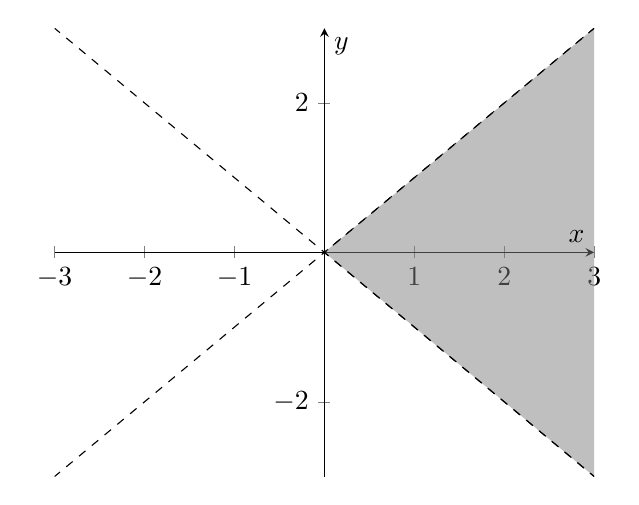
\begin{tikzpicture}
                \begin{axis}[
                    axis lines = center,
                    xlabel = \(x\),
                    ylabel = \(y\),
                    xmin = -3, xmax = 3,
                    ymin = -3, ymax = 3,
                ]
                
                \addplot [samples=2, dashed] {x};
                \addplot [samples=2, dashed] {-x};
    
                % Triangulo (4,4) (0,0) (4,-4)
                \addplot [fill=gray, fill opacity=0.5, dashed] coordinates {(4,4) (0,0) (4,-4)};
                \end{axis}
            \end{tikzpicture}
            \caption{Dominio $\Omega$ del Ejercicio~\ref{ej:3.1}.\ref{ej:3.1c}.}
            \label{fig:3.1c}
        \end{figure}

        Veamos ahora que $\Omega$ es convexo y por tanto estrellado, algo que intuitivamente podemos deducir.
        \begin{itemize}
            \item Sean $z=(x,y),~z'=(x',y')\in\Omega$, y veamos que $[z,z']\subset\Omega$.
            \begin{align*}
                [z,z']&=\{t(x,y)+(1-t)(x',y')\mid t\in[0,1]\}
                =\\&= \{(tx+(1-t)x',ty+(1-t)y')\mid t\in[0,1]\}
            \end{align*}
            \begin{itemize}
                \item Por un lado, como $x,x'>0$ y $t,1-t\geq 0$ pero no se anulan a la vez, tenemos que $tx+(1-t)x'>0$.
                \item Por otro lado, sabiendo que $-x<y<x$ y $-x'<y'<x'$, razonamos de forma directa que:
                \begin{equation*}
                    -(tx+(1-t)x')=t(-x)+(1-t)(-x')<ty+(1-t)y'<tx+(1-t)x'
                \end{equation*}
            \end{itemize}
            Por tanto, $[z,z']\subset\Omega$ y $\Omega$ es convexo.
        \end{itemize}

        Además, como los argumentos de las raíces son positivos, $P,Q\in C^1(\Omega)$. Veamos ahora si se cumple la condición de exactitud:
        \begin{align*}
            \frac{\partial P}{\partial y}(x,y) &= \frac{1}{2\sqrt{x+y}}-\frac{1}{2\sqrt{x-y}} = \frac{\partial Q}{\partial x}(x,y)
        \end{align*}

        Por tanto, existe una función potencial para este campo vectorial. Para encontrarla, como se busca que $\dfrac{\partial U}{\partial x}=P$, tenemos que:
        \begin{equation*}
            U(x,y)=\int P(x,y)dx =
            \int \sqrt{x+y}+\sqrt{x-y}dx = \frac{2}{3}(x+y)^{\nicefrac{3}{2}}+\frac{2}{3}(x-y)^{\nicefrac{3}{2}}+\varphi(y)
        \end{equation*}
        donde $\varphi:\bb{R}\to\bb{R}$ es una función que depende solo de $y$ y representa la constante de integración. Derivando $U$ respecto de $y$ obtenemos:
        \begin{align*}
            \frac{\partial U}{\partial y}(x,y)&=\sqrt{x+y}-\sqrt{x-y}+\varphi'(y) \\
            \frac{\partial U}{\partial y}(x,y)&=Q(x,y)=\sqrt{x+y}-\sqrt{x-y}
        \end{align*}

        Por tanto, $\varphi'(y)=0$. Entonces, por ejemplo, $\varphi(y)=0$. Por tanto, la función potencial es (salvo una constante aditiva):
        \begin{equation*}
            U(x,y)=\frac{2}{3}(x+y)^{\nicefrac{3}{2}}+\frac{2}{3}(x-y)^{\nicefrac{3}{2}}
        \end{equation*}
    \end{enumerate}
\end{ejercicio}

\begin{ejercicio}
    Resuelve las siguientes ecuaciones, sabiendo que admiten un factor integrante que depende de una sola de las
    variables $x$, $y$.
    \begin{enumerate}
        \item $6xy + (4y + 9x^2)y' = 0$
        
        El dominio de esta ecuación es $\Omega=\bb{R}^2$, que es abierto y conexo. Buscamos obtener un factor integrante $\mu:\Omega \to\bb{R}$. Para ello, necesitamos que se cumpla la condición de exactitud tras multiplicar por $\mu$. Definimos:
        \Func{P}{\bb{R}^2}{\bb{R}}{(x,y)}{6xy}
        \Func{Q}{\bb{R}^2}{\bb{R}}{(x,y)}{4y+9x^2}

        Calculemos las derivadas parciales implicadas en la condición de exactitud:
        \begin{align*}
            \frac{\partial (\mu P)}{\partial y} &= \dfrac{\partial \mu}{\partial y}P+\mu\dfrac{\partial P}{\partial y}\\
            \frac{\partial (\mu Q)}{\partial x} &= \dfrac{\partial \mu}{\partial x}Q+\mu\dfrac{\partial Q}{\partial x}
        \end{align*}

        Por tanto, la condición de exactitud se traduce en:
        \begin{equation*}
            \dfrac{\partial \mu}{\partial y}P- \dfrac{\partial \mu}{\partial x}Q = \mu\left(\dfrac{\partial Q}{\partial x}-\dfrac{\partial P}{\partial y}\right)
        \end{equation*}
        \item $2y \cos x - xy \sen x + (2x \cos x)y' = 0$
    \end{enumerate}
\end{ejercicio}

\begin{ejercicio}
    Encuentra $p$, $q \in \bb{R}$ para que la ecuación
    \[
        -y^2 + (x^2 + xy)y' = 0
    \]
    admita un factor integrante de la forma $\mu(x, y) = x^p y^q$. Usa dicho factor integrante para resolver la ecuación. Indica
    un método de resolución alternativo.
\end{ejercicio}

\begin{ejercicio}
    Encuentra una condición suficiente para que la ecuación $P(x, y) + Q(x, y)y' = 0$ admita un factor integrante de la
    forma $\mu(x, y) = m(xy)$. Mediante un factor integrante de este tipo, encuentra la solución general de la ecuación
    \[
        1 + xy + y^2 + (1 + xy + x^2)y' = 0.
    \]
\end{ejercicio}

\begin{ejercicio}
    Dada una función $H \in C^2(\bb{R}^2)$, $H = H(x, y)$, se considera el sistema Hamiltoniano asociado
    \[
        \begin{cases}
            \dfrac{dx}{dt} = \dfrac{\partial H}{\partial y}(x, y) \\ \\
            \dfrac{dy}{dt} = -\dfrac{\partial H}{\partial x}(x, y).
        \end{cases}
    \]
    Al tratarse de un sistema autónomo, es posible obtener la ecuación de las órbitas.
    \begin{enumerate}
        \item Demuestra que la ecuación de las órbitas se puede escribir como
        \[
            \frac{\partial H}{\partial x}(x, y) + \frac{\partial H}{\partial y}(x, y)y' = 0
        \]
        y comprueba que se trata de una ecuación exacta.
        \item Se supone que $H(x, y) = x^2 + 2y^2$. Escribe el sistema, la ecuación de las órbitas y encuentra las soluciones y
        las órbitas.
    \end{enumerate}
\end{ejercicio}

\begin{ejercicio}
    Dado un dominio $\Omega$ del plano se considera un campo vectorial $B : \Omega \to \bb{R}^2$, $B = (B_1, B_2)$, $B = B(x, y)$. Se supone
    $B \in C^1(\Omega, \bb{R}^2)$. Diremos que $B$ es un campo solenoidal si se cumple
    \[
        \text{div } B := \frac{\partial B_1}{\partial x} + \frac{\partial B_2}{\partial y} = 0,
    \]
    donde $\text{div}$ es el operador divergencia.
    \begin{enumerate}
        \item Determina los valores de las constantes $a$, $b$, $c$, $d$ para los que el campo $B(x, y) = (ax+by, cx+dy)$ es solenoidal.
        \item Demuestra que si el dominio $\Omega$ tiene forma de estrella entonces para cada campo solenoidal $B$ existe una
        función $A \in C^2(\Omega)$ tal que $\frac{\partial A}{\partial x} = B_2$, $\frac{\partial A}{\partial y} = -B_1$.
    \end{enumerate}
\end{ejercicio}

\begin{ejercicio}
    Se considera un campo de fuerzas $F : \bb{R}^3 \to \bb{R}^3$, $F = (F_1, F_2, F_3)$, $F = F(x, y, z)$, de clase $C^1$.
    \begin{enumerate}
        \item Demuestra que existe una función $U \in C^2(\bb{R}^3)$ que cumple $\frac{\partial U}{\partial x} = F_1$,
        $\frac{\partial U}{\partial y} = F_2$, $\frac{\partial U}{\partial z} = F_3$ si y solo si se cumplen
        las condiciones de exactitud
        \[
            \frac{\partial F_1}{\partial y} = \frac{\partial F_2}{\partial x}, \quad
            \frac{\partial F_1}{\partial z} = \frac{\partial F_3}{\partial x}, \quad
            \frac{\partial F_2}{\partial z} = \frac{\partial F_3}{\partial y}.
        \]
        \item Generalización a $\bb{R}^d$.
    \end{enumerate}
\end{ejercicio}

\begin{ejercicio}
    Se considera un campo de fuerzas $F : \bb{R}^2 \to \bb{R}^2$, $F = (F_1, F_2)$, $F = F(x, y)$, de clase $C^1$. Se define la función
    $T : \bb{R}^2 \to \bb{R}$, $T = T(x, y)$ como el trabajo realizado a lo largo del camino $\gamma(t) = (tx, t^2y)$, $t \in [0, 1]$.
    \begin{enumerate}
        \item Demuestra que $T$ es una función de clase $C^1$.
        \item Calcula las derivadas parciales de $T$.
        \item Se define ahora $\wt{T}$ como el trabajo realizado a lo largo del camino $\wt{\gamma}(t) = (t^2x, ty)$, $t \in [0, 1]$. ¿Se puede asegurar
        que $T$ y $\wt{T}$ coinciden?
    \end{enumerate}
\end{ejercicio}